\documentclass[11pt]{article}

\usepackage{dirtree}
\usepackage{lmodern}
\usepackage{listings}
\usepackage{color}
\usepackage{tikz}

\usepackage{graphicx}    % needed for including graphics e.g. EPS, PS
\usepackage{epstopdf}
\usepackage{amsmath}
\usepackage{hyperref}
\usepackage{xspace}
\usepackage{mathtools}
\usepackage{epsfig}
\usepackage{float}
\usepackage{natbib}
\usepackage{subfigure}
\usepackage{setspace}
\usepackage{tabularx,ragged2e,booktabs,caption}

\setlength{\topmargin}{-1in}     %\topmargin: gap above header
%\setlength{\columnsep}{0in}      %\columnsep: gap between columns
\setlength{\headheight}{0in}     %\headheight: height of header
\setlength{\topskip}{0in}        %\topskip: between header and text
\setlength{\headsep}{0in}        
\setlength{\textheight}{692pt}   %\textheight: height of main text
\setlength{\textwidth}{7.5in}    % \textwidth: width of text
\setlength{\oddsidemargin}{-0.5in}  % \oddsidemargin: odd page left margin
\setlength{\evensidemargin}{0in} %\evensidemargin : even page left margin
\setlength{\parindent}{0.25in}   %\parindent: indentation of paragraphs
\setlength{\parskip}{0pt}        %\parskip: gap between paragraphs
\setlength{\voffset}{0.5in}


\newcommand{\eqtab}{\;\;\;\;\;\;\;\;\;\;\;\;\;\;\;\;}
\newcommand{\divBz}{$\nabla \bullet B = 0$}
\newcommand{\divB}{$\nabla \bullet B$}
\newcommand{\Rem}{$Re_m$}
\newcommand{\jcrossB}{$j \times B$}

%\newcommand{\figW}{6.5in}
%\newcommand{\figH}{5.5in}
\newcommand{\figW}{5.in}
\newcommand{\figH}{4.in}
%\newcommand{\figW}{6.825in}
%\newcommand{\figH}{5.775in}

\newcommand{\ffigW}{3.1in}
\newcommand{\ffigH}{3.1in}

\lstset{language=[90]Fortran,
  basicstyle=\ttfamily,
  keywordstyle=\color{red},
  commentstyle=\color{green},
  morecomment=[l]{!\ }% Comment only with space after !
}

\begin{document}
\doublespacing
\begin{figure}
\centering
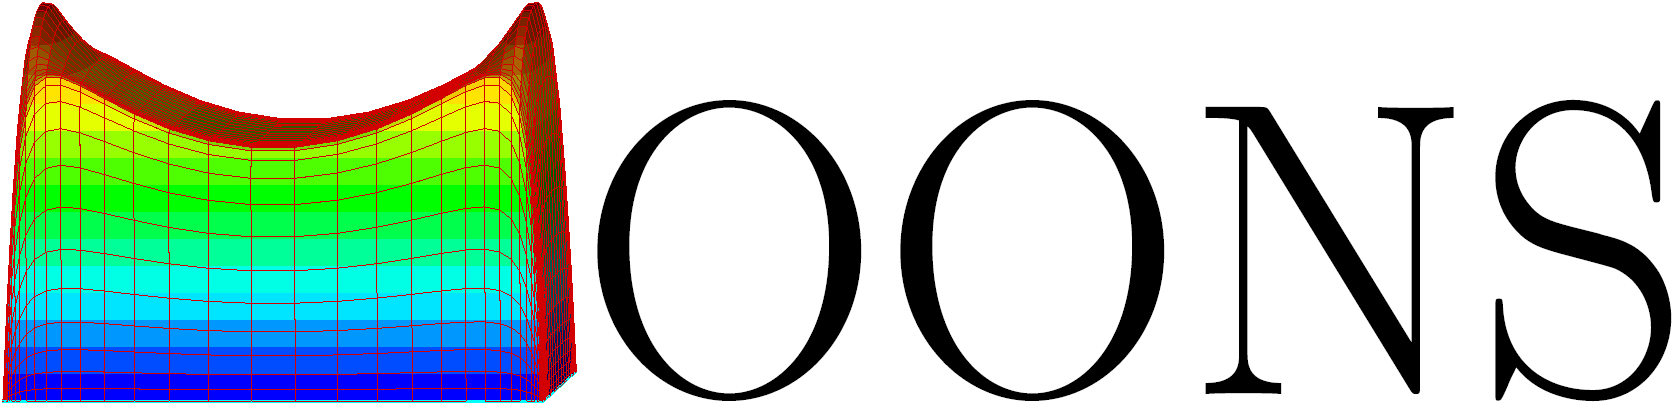
\includegraphics[width=3in,height=0.8in]{MOONS_logo.png}
\end{figure}
\title{Magnetohydrodynamic Object-Oriented Numerical Solver (MOONS)}
\author{C. Kawczynski \\
Department of Mechanical and Aerospace Engineering \\
University of California Los Angeles, USA\\
}
\maketitle

\begin{abstract}
UCLA has developed a Magnetohydrodynamic Object-Oriented Numerical Solver (MOONS) finite difference code. This report is an attempt to document 1) the governing equations that MOONS solves 2) techniques that MOONS implements when solving solving these equations 3) ideas that have been used to develop MOONS 4) benchmarks that MOONS has performed. 5) provide a low barrier to entry to new users.
\end{abstract}

\section{Introduction}
The purpose of MOONS was to compare a small research code with a commercial code, HIMAG, developed by HyperComp with help from UCLA. A new formulation was being implemented in HIMAG, and MOONS was developed to compare the old and new version of HIMAG for simple test cases that MOONS could handle. There are derivations of selected equations in the documentation section of MOONS.

\section{Governing Equations}

\subsection{Momentum}
The momentum equation is solved using the same numerical techniques as described in \cite{griebel1997numerical}.
Non-dimensionalizing the momentum equation with
\begin{equation*}
U_i^* = U_i/U_c  \eqtab
\nabla^* = L_c \nabla \eqtab
t^* = t/t_c  \eqtab
t_c = L_c/U_c
\end{equation*}

Yields the dimensionless momentum equation. Removing the asterisks for simplicity, the momentum equation is

\begin{equation} \label{eq:momentum}
\frac{\partial \pmb{u}}{\partial t} = 
- ( \pmb{u} \bullet \nabla ) \pmb{u}
- \nabla p
+ Re^{-1} \nabla^2 \pmb{u} 
+ \frac{L_c}{\rho_c U_c^2} \pmb{f}
+ \frac{Ha^2}{Re} \pmb{j} \times \pmb{B}
\end{equation}
Or, using index notation, the ith component is
\begin{equation} \label{eq:momentumIndex}
\partial_t u_i = 
- u_j \partial_j u_i 
- \partial_i p 
+ Re^{-1} \partial_j \partial_j u_i 
+ \frac{L_c}{\rho_c U_c^2} f_i
+ \frac{Ha^2}{Re} \epsilon_{imn} j_m B_n
\end{equation}

\begin{equation} \label{eq:Re}
Re = \frac{U_c L_c}{\nu_c}
\eqtab
Ha = B_c L_c \sqrt{\sigma_c/\mu_c}
\end{equation}

Where $f_i$ is some dimensional force per unit volume along the ith direction. The advective term can be treated in one of two ways.

1) Conservative, Donor-cell form (neglecting sign):
\begin{equation} \label{eq:Donor-Cell}
\partial_j (u_j u_i)
\end{equation}

2) Advective form (neglecting sign)
\begin{equation} \label{eq:advectiveUForm}
u_{j,ave} \partial_j u_i
\end{equation}

This can be specified in user/simParams.f90

\subsection{Full Induction}
Solving for the electric field in Ohm's law, and the current in Ampere's law, and combining them with Faraday's law yields the induction equation. Non-dimensionalizing the induction equation with the same characteristic values from above as well as
\begin{equation*}
B_i^* = B_i/B_c  ,\eqtab
\sigma^* = \sigma/\sigma_c ,\eqtab
\mu^* = \mu/\mu_c ,\eqtab
E_i^* = E_i/(U_c B_c) ,\eqtab
j_i^* = \frac{j}{B_i/(\mu_c L_c)}
\end{equation*}

Yields the dimensionless induction equation. Removing the asterisks for simplicity we have

\begin{equation} \label{eq:fullInduction}
\frac{\partial \pmb{B}}{\partial t} =
 \nabla \times (\pmb{u} \times \pmb{B})
- \frac{1}{Re_m} \nabla \times \left( \frac{1}{\sigma} \nabla \times \frac{\pmb{B}}{\mu} \right)
\end{equation}
With the constraint
\begin{equation} \label{eq:divB}
\nabla \bullet \pmb{B} = \pmb{0}
\end{equation}
Or
\begin{equation} \label{eq:Faraday}
\frac{\partial \pmb{B}}{\partial t} =
 - \nabla \times \pmb{E}
, \eqtab
 \pmb{E} = \frac{1}{Re_m} \frac{\pmb{j}}{\sigma} - \pmb{u} \times \pmb{B}
\end{equation}

Using index notation and the Kronecker Delta identity, we may rewrite our diffusion and advection terms:

\begin{equation*}
\nabla \times (\pmb{u} \times \pmb{B}) = -\partial_j (u_j B_i - u_i B_j), \eqtab
\frac{1}{Re_m} \nabla \times \left( \frac{1}{\sigma} \nabla \times \frac{B}{\mu} \right) = 
\frac{1}{Re_m} \partial_j \left( \frac{1}{\sigma} \left[ \partial_i \frac{B_j}{\mu} - \partial_j \frac{B_i}{\mu} \right] \right)
\end{equation*}

So the ith component of the induction equation is

\begin{equation} \label{eq:conservativeFormulation}
 \partial_t B_i = 
-\partial_j (u_j B_i - u_i B_j)
-\frac{1}{Re_m} \partial_j \left( \frac{1}{\sigma} \left[ \partial_i \frac{B_j}{\mu} - \partial_j \frac{B_i}{\mu} \right] \right)
\end{equation}

Where
\begin{equation} \label{eq:Rem}
Re_m = \frac{U_c L_c}{(\mu_c \sigma_c)^{-1}}
\end{equation}
Note that the subscript c indicates a 'characteristic' uniform, time-independent, constant. Also note, the dimensionless material properties, $\sigma$ and $\mu$, in these equations may vary, in general, in space and or time.

\subsection{Low Magnetic Reynolds Number approximation}
Multiplying \ref{eq:conservativeFormulation} by \Rem\ and setting \Rem to zero results in only the diffusion term for the induced field and only the advection term for the applied field. Combining these two results, and introducing a pseudo time-stepping, we may write this as

\begin{equation} \label{eq:LowRemPsuedo}
\partial_s B_i = -\partial_j (u_j B_i^0 - u_j B_i^0)
-\frac{1}{Re_m} \partial_j \left( \frac{1}{\sigma} \left[ \partial_i \frac{B_j}{\mu} - \partial_j \frac{B_i}{\mu} \right] \right)
\end{equation}

Where $B$ and $B^0$ are the induced and applied magnetic fields and $s$ is a pseudo time step used to solve the steady state BVP. For uniform properties, this may simplify, by applying $\partial_j B_j = 0$ to the diffusion term after exchanging the order of derivatives, to the Poisson equation

\begin{equation} \label{eq:LowRemPoisson}
\partial_j \partial_j B_i = \partial_j (u_j B_i^0 - u_i B_j^0)
\end{equation}

\subsection{Divergence of the Magnetic Field}
The divergence B constraint, \ref{eq:divB}, is not naturally satisfied when solving the full induction equation and requires special care to be enforced. MOONS offers several options to handle this constraint and they are discussed in the next subsections.

\subsubsection{Constrained Transport (CT) method}
The CT method enforces \ref{eq:divB} within machine accuracy at every time step so long the applied magnetic field also satisfies \ref{eq:divB}. This is accomplished by solving \ref{eq:Faraday} where the electric field is carefully defined such that there is a perfect numerical cancellation of the divergence of B \cite{Toth2000}.

\subsubsection{Brackbill - Projection method}
One cleaning procedure that has been implemented was performed by \citep{Brackbill1980}. This method is a projection method where the solution of the induction equation is a sub-step, and then subtracting the gradient of potential field, $\phi$ results in the 'cleaned' magnetic field:
\begin{equation}  \label{eq:Projection}
\pmb{B}^{n+1} = \pmb{B}^* - \nabla \phi
\end{equation}
Where $\phi$ satisfies Poisson equation:
\begin{equation} 
\nabla^2 \phi = \nabla \bullet \pmb{B}^*
\end{equation}
And $\pmb{B}^*$ is the magnetic field solved from \ref{eq:fullInduction} or \ref{eq:conservativeFormulation}.

\subsubsection{No treatment}
In some cases, the numerical divergence of the Magnetic field is small and has no significant effect on the fluid flow. In these cases, it may be more advantageous to avoid any sort of cleaning or staggered variables to enforce \ref{eq:divB} at all.


\subsection{Material properties}
To treat the interface between the liquid and solid domain, the approach in \cite{Carvalho2013} was adopted. At the interface, a harmonic weighting function was used to described the transition of the changing material properties:
\begin{equation*}
\sigma^*_{interface} = \frac{\sigma}{\sigma_l} = \frac{2 \sigma_w}{\sigma_w + \sigma_l}
\end{equation*}


\subsection{Boundary conditions}
MOONS implements a class called BCs to package BCs for any particular solver. Then, the routine applyAllBCs is used to assign the appropriate BCs. BCs are implemented for 1st and 2nd order accuracy for collocated and staggered grids. If a variable is not coincident with the wall where you wish to enforce a particular BC, then it includes the interpolation such that the BC is satisfied at the wall. 

\subsubsection{Velocity Field}
MOONS has a simple interface for enforcing the following BCs

No slip / no flow through (Dirichlet) and Fully developed (Neumann)
\begin{equation*}
\pmb{u} = \pmb{u}_{b} \eqtab
\pmb{u} = \pmb{0} \eqtab
\partial_n \pmb{u}_n = 0
\end{equation*}

\subsubsection{Magnetic Field}
By default, MOONS implements Fluent-Type BCs for the magnetic field:
\begin{equation*} 
\left( \frac{\partial \pmb{B}_{normal}}{\partial n} \right)_{boundary} = 0 \eqtab
\pmb{B}_{tangential} = 0
\end{equation*}

If a cleaning procedure is used to enforce \divBz\, then the BCs for the scalar potential are
\begin{equation*}
\left(\frac{\partial \phi}{\partial n} \right)_{boundary} = 0
\end{equation*}

\subsubsection{applying BCs in MOONS}
In order to assign BCs for the Ufield or Bfield, navigate to the user/initialize/momentum or /user/initialize/induction respectively. This is where the BCs are assigned for the velocity and magnetic field. The module computations/applyBCs.f90 specifies the stencils for all boundary conditions. They include stencils for collocated and staggered grids, meaning that if a variable is not coincident with the wall where you wish to enforce a particular BC, then it includes the interpolation such that the BC is satisfied at the wall. Looking at /static/BCs.f90 and applyBCs.f90 should help understand how to create the derived type, 'BCs', which are used in all of the solvers.

Since the velocity field is solved on a staggered grid, the BCs for wall-normal and wall-tangent components are different.

\section{Solvers}
\subsection{Momentum}
\subsection{Induction}
\subsection{Poisson}
\subsubsection{SOR / Gauss Seidel}
The relaxation parameter was determined by

\begin{equation} \label{eq:RelaxationParam}
\omega_{opt} = \frac{2}{1 + \sqrt{1 - \rho^2}}
\end{equation}

Where $\rho$ is the spectral radius of the iteration matrix of the Jacobi method \cite{Yang2009}. For a 1D and 2D grids, the optimal parameter may be calculated as \cite{Mcdonough2008}

\begin{equation}
\omega_{opt,1D} = \frac{2}{1 + \sqrt{1 - \left( \frac{\cos\left(\frac{\pi}{N_x+1} \right)}{1} \right)^2}}
\end{equation}

\begin{equation}
\omega_{opt,2D} = \frac{2}{1 + \sqrt{1 - \left( \frac{\cos\left(\frac{\pi}{N_x+1} \right) + \cos\left(\frac{\pi}{N_y+1} \right)}{2} \right)^2}}
\end{equation}

respectively. The following has not been found in literature, but MOONS implements the following optimal parameter for the 3D simulations:

\begin{equation}
\omega_{3D} = \frac{2}{1 + \sqrt{1 - \left( \frac{\cos\left(\frac{\pi}{N_x+1} \right) + \cos\left(\frac{\pi}{N_y+1} \right)+ \cos\left(\frac{\pi}{N_z+1} \right)}{3} \right)^2}}
\end{equation}

There is a logical parameter in SOR.f90 to use Gauss Seidel, which sets $\omega=1$.

\subsubsection{Multigrid}
MOONS has an unfinished geometric multigrid. There are many restrictions and prolongations required for the MG method, and implementing this routine has not been my top priority.

\subsection{Root Solver}
MOONS implements a root solver in order to estimate matching the interior cell size with the first exterior wall cell size. This is done by matching the interior stretching factor, $\beta_i$, with the stretching factor in the wall $\beta_w$. Currently, the root solver currently defines a vector of the roots, takes the absolute value of the vector, then locates the minimum. I believe it may be better to implement Newton's method in the future. The only issue I see with using Newtons method is that there are asymptotic bounds in the root that may cause problems with using Newton's method. The current method avoids this by ensuring that not too large and not too small values are chosen. Also, the root solver need not be exact, since it is only used to determine the cell nodes (corners) after the first exterior cell.

\section{Modules}

\section{Mesh}
The mesh created was using a Robert's stretching function defined in \cite{pletcher2012computational}. 

MOONS automatically ensures that the size of the first exterior (wall) cell is the same exact size as the first interior fluid cell. This is important because MOONS extrapolates any data using a linear extrapolation, which assumes that the cells are the same size. This means special treatment would be required for extrapolated data to be consistent with, for example, the forcing term in the Poisson equation for pressure or for the magnetic field if the low \Rem approximation is being used.

MOONS also uses a few checks to make sure that prescribed inputs are consistent. For example, if the wall thickness is zero, then the number of cells in the wall better be zero. If inconsistent problems like these are found, MOONS stops the simulation before it even starts and reports the error.

\section{Errors}
The MOONS error module calculates several errors including $L_1$,$L_2$ and $L_{\infty}$ norms. The following sections show the details of these calculations. They are performed in /computations/myError.f90

\subsection{Absolute}
\begin{equation}
L_n(f_{exact},f) =  \sqrt[n]{\sum_{i,j,k} |(f_{exact})_{i,j,k} - f_{i,j,k}|^n} \eqtab
L_\infty(f_{exact},f) = \max( (f_{exact}) - f )
\end{equation}

\subsection{Relative}
\begin{equation}
R_{n}(f_{exact},f) = \frac{L_n(f_{exact},f)}{L_n(f_{exact},0)} \eqtab
R_{\infty}(f_{exact},f) = \frac{L_\infty(f_{exact},f)}{L_\infty(f_{exact},0)}
\end{equation}

Note that when $f_{exact}$ is less than a tolerance of $10^{-6}$ everywhere, 1 is added to the denominator to avoid division by zero, which results in

\begin{equation}
R_{n}(f_{exact},f) = L_n(f_{exact},f) \eqtab
R_{\infty}(f_{exact},f) = L_\infty(f_{exact},f)
\end{equation}

\section{Parallelization}
MOONS is openMP parallel ready. In gfortran, the -fopenmp flag must be used. In addition to the compiler flag, useOpenMP must be set to .true. in user/simParams.f90 to solve the Poisson Equation in parallel. The reason for this is that the Poisson loop was split into two loops for parallelization, and the single loop may run faster in serial.

MOONS has parallelization for the following routines:

\begin{lstlisting}
    interpO2()         (/computations/vectorOps.f90)
    myDell()           (/computations/myDel.f90)
    mySOR()            (/solvers/steadyState/SOR.f90)
    myError()          (/computations/myError.f90)
\end{lstlisting}

\section{Directionality}
MOONS computes derivatives, interpolates, and is indexed in the same way for all three directions. Implementing directionless routines was a highly sought task when implementing MOONS and has paid off greatly in the simplicity of implementation. Furthermore, the explanation of these routines will be described in 1D for succinctness.

\section{Derivatives, Interpolations and BC formulas}
\subsection{Derivatives}

\subsection{Interpolations}

\subsection{BC formulas}


\section{Indexing}

MOONS indexes starting from 1. This was a carefully chosen decision because with the indexing starting from 1, the Fortran intrinsic \lstinline$shape()$ can be used to obtain the size of the incoming data in a subroutine and internally decide where the data lives based on the dimensions.

The index convention has been drawn in a diagram below.
\begin{figure}[h!]
  \begin{center}
    \begin{tikzpicture}
      \draw [thick] (0,0) to (4,0);
      \draw [thick,dashed] (4,0) to (6,0);
      \draw [thick] (6,0) to (10,0);

      \draw [black] (0,0) circle [radius=0.1];
      \draw [radius=0.1] (0,0) node [black,below=12] {$f_{1}$};

      \draw [thick] (1,-0.3) to (1,0.3);

      \draw [black] (2,0) circle [radius=0.1];
      \draw [radius=0.1] (2,0) node [black,below=12] {$f_{2}$};

      \draw [thick] (3,-0.3) to (3,0.3);

      \draw [thick] (7,-0.3) to (7,0.3);

      \draw [black] (8,0) circle [radius=0.1];
      \draw [radius=0.1] (8,0) node [black,below=12] {$f_{N+1}$};

      \draw [thick] (9,-0.3) to (9,0.3);

      \draw [black] (10,0) circle [radius=0.1];
      \draw [radius=0.1] (10,0) node [black,below=12] {$f_{N+2}$};

    \end{tikzpicture}
    \caption{Index convention for cell center / edge data}
  \end{center}
\end{figure}

\begin{figure}[h!]
  \begin{center}
    \begin{tikzpicture}
      \draw [thick] (0,0) to (4,0);
      \draw [thick,dashed] (4,0) to (6,0);
      \draw [thick] (6,0) to (10,0);

      \draw [thick] (0,-0.3) to (0,0.3);
      \draw [radius=0.1] (0,0) node [black,below=12] {$f_{1}$};

      \draw [black] (1,0) circle [radius=0.1];

      \draw [thick] (2,-0.3) to (2,0.3);
      \draw [radius=0.1] (2,0) node [black,below=12] {$f_{2}$};

      \draw [thick] (8,-0.3) to (8,0.3);
      \draw [radius=0.1] (8,0) node [black,below=12] {$f_{N}$};

      \draw [black] (9,0) circle [radius=0.1];

      \draw [thick] (10,-0.3) to (10,0.3);
      \draw [radius=0.1] (10,0) node [black,below=12] {$f_{N+1}$};

    \end{tikzpicture}
    \caption{Index convention for node / face centered data}
  \end{center}
\end{figure}

Where $N$ is the number of $cells$ in the domain (interior or total depending on the field in question).

\section{Running MOONS}
In order to run MOONS, you'll need to call MOONS from a project directory. The only input to calling MOONS is the output directory.

\begin{lstlisting}
       include 'includes.f90'
       program runMoons
       use MOONS_mod
       implicit none
       call MOONS('out\LidDrivenCavity\')
       end program
\end{lstlisting}

Before running MOONS, your project directory may look something like this:

\dirtree{%
.1 Project/.
.2 bin.
.2 main.f90.
}

After running MOONS, your directory tree should looks like this

\dirtree{%
.1 Project/.
.2 bin.
.2 main.f90.
.2 out.
.3 LidDrivenCavity.
.4 BField.
.4 JField.
.4 material.
.4 parameters.
.4 UField.
.4 CPU TIME INFO.dat.
}

\subsection{Post Processing}
Once MOONS has finished running, navigate to /MATLAB/MOONS/main.m and run with the appropriate settings. Once doing this, each field folder in your directory tree should have a new folder named 'figs' which will contain the output plots of MOONS.


\section{Running a simple simulation}
Let's set up the benchmark problem 1. A Lid Driven Cavity flow for Re=400, Ha=0.
The following table shows which parameters are in which files and the values you must set them to.

\begin{table}[h]
\begin{tabular}{lllll}
griddata.f90 &  &  &  &  \\
 &  &  &  &  \\
 &  &  &  &  \\
 &  &  &  & 
\end{tabular}
\end{table}


\subsection{Setting parameters}

\subsection{Compile}

\subsection{Run}

\subsection{Post Processing}


\section{Benchmarks}

\subsection{Lid Driven Cavity Flow}


\subsection{Square Duct Flow}

\section{Navigating MOONS}
A large effort in developing MOONS was to ensure that the code, organization, and logic is highly transparent. Look at the directory tree, it shouldn't take more than a few seconds to find which folder the momentum solver is located. The idea of transparency also holds in the individual files themselves. If a subroutine or function seems opaque, there should be documentation explaining what it's doing, otherwise, it should be relatively self-explanatory by the name of the subroutine.

\subsection{Directory Tree}
Below is the MOONS directory tree, showing the location of the modules and solvers for the user to set parameters for a simulation.

\dirtree{%
.1 MOONS/.
.2 documentation.
.3 MOONS.pdf (this file).
.3 Derivations.
.4 Non-uniform Grid Stencil.pdf.
.2 solvers.
.3 steadyState.
.4 Poisson.f90.
.4 SOR.f90.
.4 MG.f90 (not finished).
.3 transient.
.4 MHDSolver.f90.
.4 ADI.f90 (not finished).
.4 momentum.
.5 momentumSolver.f90.
.4 induction.
.5 inductionSolver.f90.
.2 static \ldots{} \begin{minipage}[t]{10cm} Auxiliary files, no settings exist here
\end{minipage}.
.2 matlab.
.3 plotResults\ldots{} \begin{minipage}[t]{10cm} matlab plotting files \end{minipage}.
.3 tools\ldots{} \begin{minipage}[t]{10cm} matlab tools for plotting \end{minipage}.
.3 main.m.
.3 benchmarking.m.
.2 user.
.3 initialize.
.4 momentum.
.5 initializeUBCs.f90.
.5 initializeUField.f90.
.4 induction.
.5 initializeBBCs.f90.
.5 initializeBField.f90.
.5 initializeSigmaMu.f90.
.3 constants.f90 - sets precision etc.
.3 griddata.f90 - sets geometry, N cells, $t_w$, stretching etc. 
.3 MOONS.f90 - sets $Re$, $Ha$, $Re_m$ etc.
.3 rundata.f90  - sets $\Delta t$ etc.
.3 simParams.f90 - sets equations to solve, how to solve them (coupled/uncoupled) etc.
.2 includes.f90 - specifies files for MOONS to include.
}



\bibliographystyle{unsrt}
\bibliography{MHD,Math,Interface,fluids,CFD,handpicked}

\end{document}